\chapter{The final application}
\label{chap:ch4}

\par The application, called \href{https://github.com/solomonarul/edra}{\texttt{Edra}}, has been designed from the outset with a primary focus on performance, emphasizing both speed and low latency. To meet these requirements, the C programming language was selected for the development of the emulator, due to its low-level access to system resources and minimal runtime overhead.

\par For graphical output and user interaction, the \href{https://wiki.libsdl.org/SDL3/FrontPage}{\texttt{SDL3}} library was chosen for its cross-platform compatibility, lightweight nature, and ease of integration into C-based projects.

\par When evaluating options for graphical user interface (GUI) development in pure C, the available choices were rather limited. The GUI development space is predominantly occupied by C++ libraries such as \href{https://github.com/ocornut/imgui}{\textit{ImGui}}, which are not directly compatible with C without the use of external bindings which would make the development process rather complicated.

\par Ultimately, the project adopted the \href{https://github.com/nicbarker/clay}{\texttt{clay}} library, a platform-agnostic C layout engine. This library facilitates GUI construction by generating a series of rendering operations that can be implemented using a backend such as \href{https://wiki.libsdl.org/SDL3/FrontPage}{\texttt{SDL3}}, thereby enabling flexible and portable UI rendering within the application.

\section{Design and implementation}
\label{sec:ch4sec1}

\par The emulator's core functionality was subsequently modularized into a dedicated git submodule, referred to as \href{https://github.com/solomonarul/cchip8}{\texttt{cchip8}}, located in the \textit{lib/cchip8} directory. This module encapsulates all fundamental components required for CHIP8 emulation.

\par Building upon this foundation, the CHIP8 driver, located in \textit{drivers/chip8}, instantiates a machine capable of loading and executing CHIP8 programs.

\par This virtual machine is then integrated into an application state, which is responsible for managing its output within the broader context of \href{https://github.com/solomonarul/edra}{\texttt{Edra}}'s state management system.

\par Similarly, the Brainfuck emulator has its own module called \href{https://github.com/solomonarul/cbf}{\texttt{cbf}} available at \textit{lib/cbf} which handles all of the components necessary for the machine at \textit{drivers/cbf} which is then used by the state in the app.

\par For cross-platform non-standard features, such as dynamic arrays, .ini file parsing and so on, custom implementations have been made and separated into their own separate module called \href{https://github.com/solomonarul/auxum}{\texttt{auxum}} available in the \textit{lib/auxum} folder.

\begin{figure}[htbp]
\centering
\begin{tikzpicture}[
    state/.style={rectangle, draw, thick, minimum width=3cm, minimum height=1cm, align=center},
    arrow/.style={-Stealth, thick}
]

% Initial state
\node[state] (initial) {\texttt{chip8\_state\_t}};
\node[below=0.2cm of initial] (label1) {Initial State};

% Pressing Enter
\node[above=1.2cm of initial] (action1) {Pressing Escape};
\draw[arrow] (initial.north) -- (action1.south);

% Paused state
\node[state, above=1cm of action1] (paused) {\texttt{chip8\_pause\_state\_t}};
\node[state, below=0.1cm of paused] (initial2) {\texttt{chip8\_state\_t}};
\node[right=0.2cm of initial2] (label2) {Paused State};

% Pressing Esc
\node[above=1.2cm of paused] (action2) {Pressing Escape};
\draw[arrow] (paused.north) -- (action2.south);

% Return to initial
\node[state, above=1cm of action2] (final) {\texttt{chip8\_state\_t}};
\node[below=0.2cm of final] (label3) {Initial State Restored};

% Return arrow
\draw[arrow, dashed] (final.east) to[out=0, in=0, looseness=1.5] (initial.east);

\end{tikzpicture}
\caption{Stack-based state transitions, as used in the app.}\label{fig:state_stack}
\end{figure}

\section{Porting and compiling}
\label{sec:ch4sec2}

\par During cross-platform porting efforts, several implementation constraints necessitated platform-specific adaptations:
\begin{itemize}
    \item \textit{PlayStation Vita}: JIT emulation was disabled due to the absence of POSIX-compliant threading support, which prevented successful compilation of the GNU Lightning library. Additionally, memory allocation thresholds required modification within the VitaSDK framework, as implemented in \href{https://github.com/solomonarul/auxum/blob/main/inc/auxum/platform/vita/heap.h}{\texttt{auxum}.}
    \item \textit{Microsoft Windows}: JIT functionality was similarly disabled following segmentation faults during compilation attributed to GNU Lightning incompatibilities, potentially stemming from toolchain limitations within the GCC Windows environment.
    \item \textit{Linux}: Full functionality was maintained without modification, demonstrating native compatibility with the implementation's architectural dependencies.
\end{itemize}

\par To facilitate compilation, a standardized build system was implemented using \texttt{Make}. This system provides template commands for all supported platforms, as documented in the project's \href{https://github.com/solomonarul/edra}{\texttt{GitHub repository}}:

\begin{enumerate}
    \item \textit{Environment Configuration}: Specify \texttt{SDL3\_DIR} and \texttt{SDL3\_TTF\_DIR} variables in CMake's build cache when required for dependency resolution.
    
    \item \textit{Platform-Specific Compilation}: Execute the appropriate build command:\\\textit{  make b\{platform\}\{configuration\}}
    \begin{itemize}
        \item \texttt{platform} denotes the target system:
        \begin{itemize}
            \item \texttt{w}: Microsoft Windows
            \item \texttt{u}: Unix-like systems (Linux, BSD)
            \item \texttt{v}: PlayStation Vita
        \end{itemize}
        \item \texttt{configuration} specifies the build type:
        \begin{itemize}
            \item \texttt{d}: Debug build
            \item \texttt{r}: Release build
        \end{itemize}
    \end{itemize}
\end{enumerate}

\clearpage

\section{Usage}
\label{sec:ch4sec3}

\subsubsection{GUI}
\label{sec:ch4sec4subsub1}

\begin{minipage}{\linewidth}
\centering
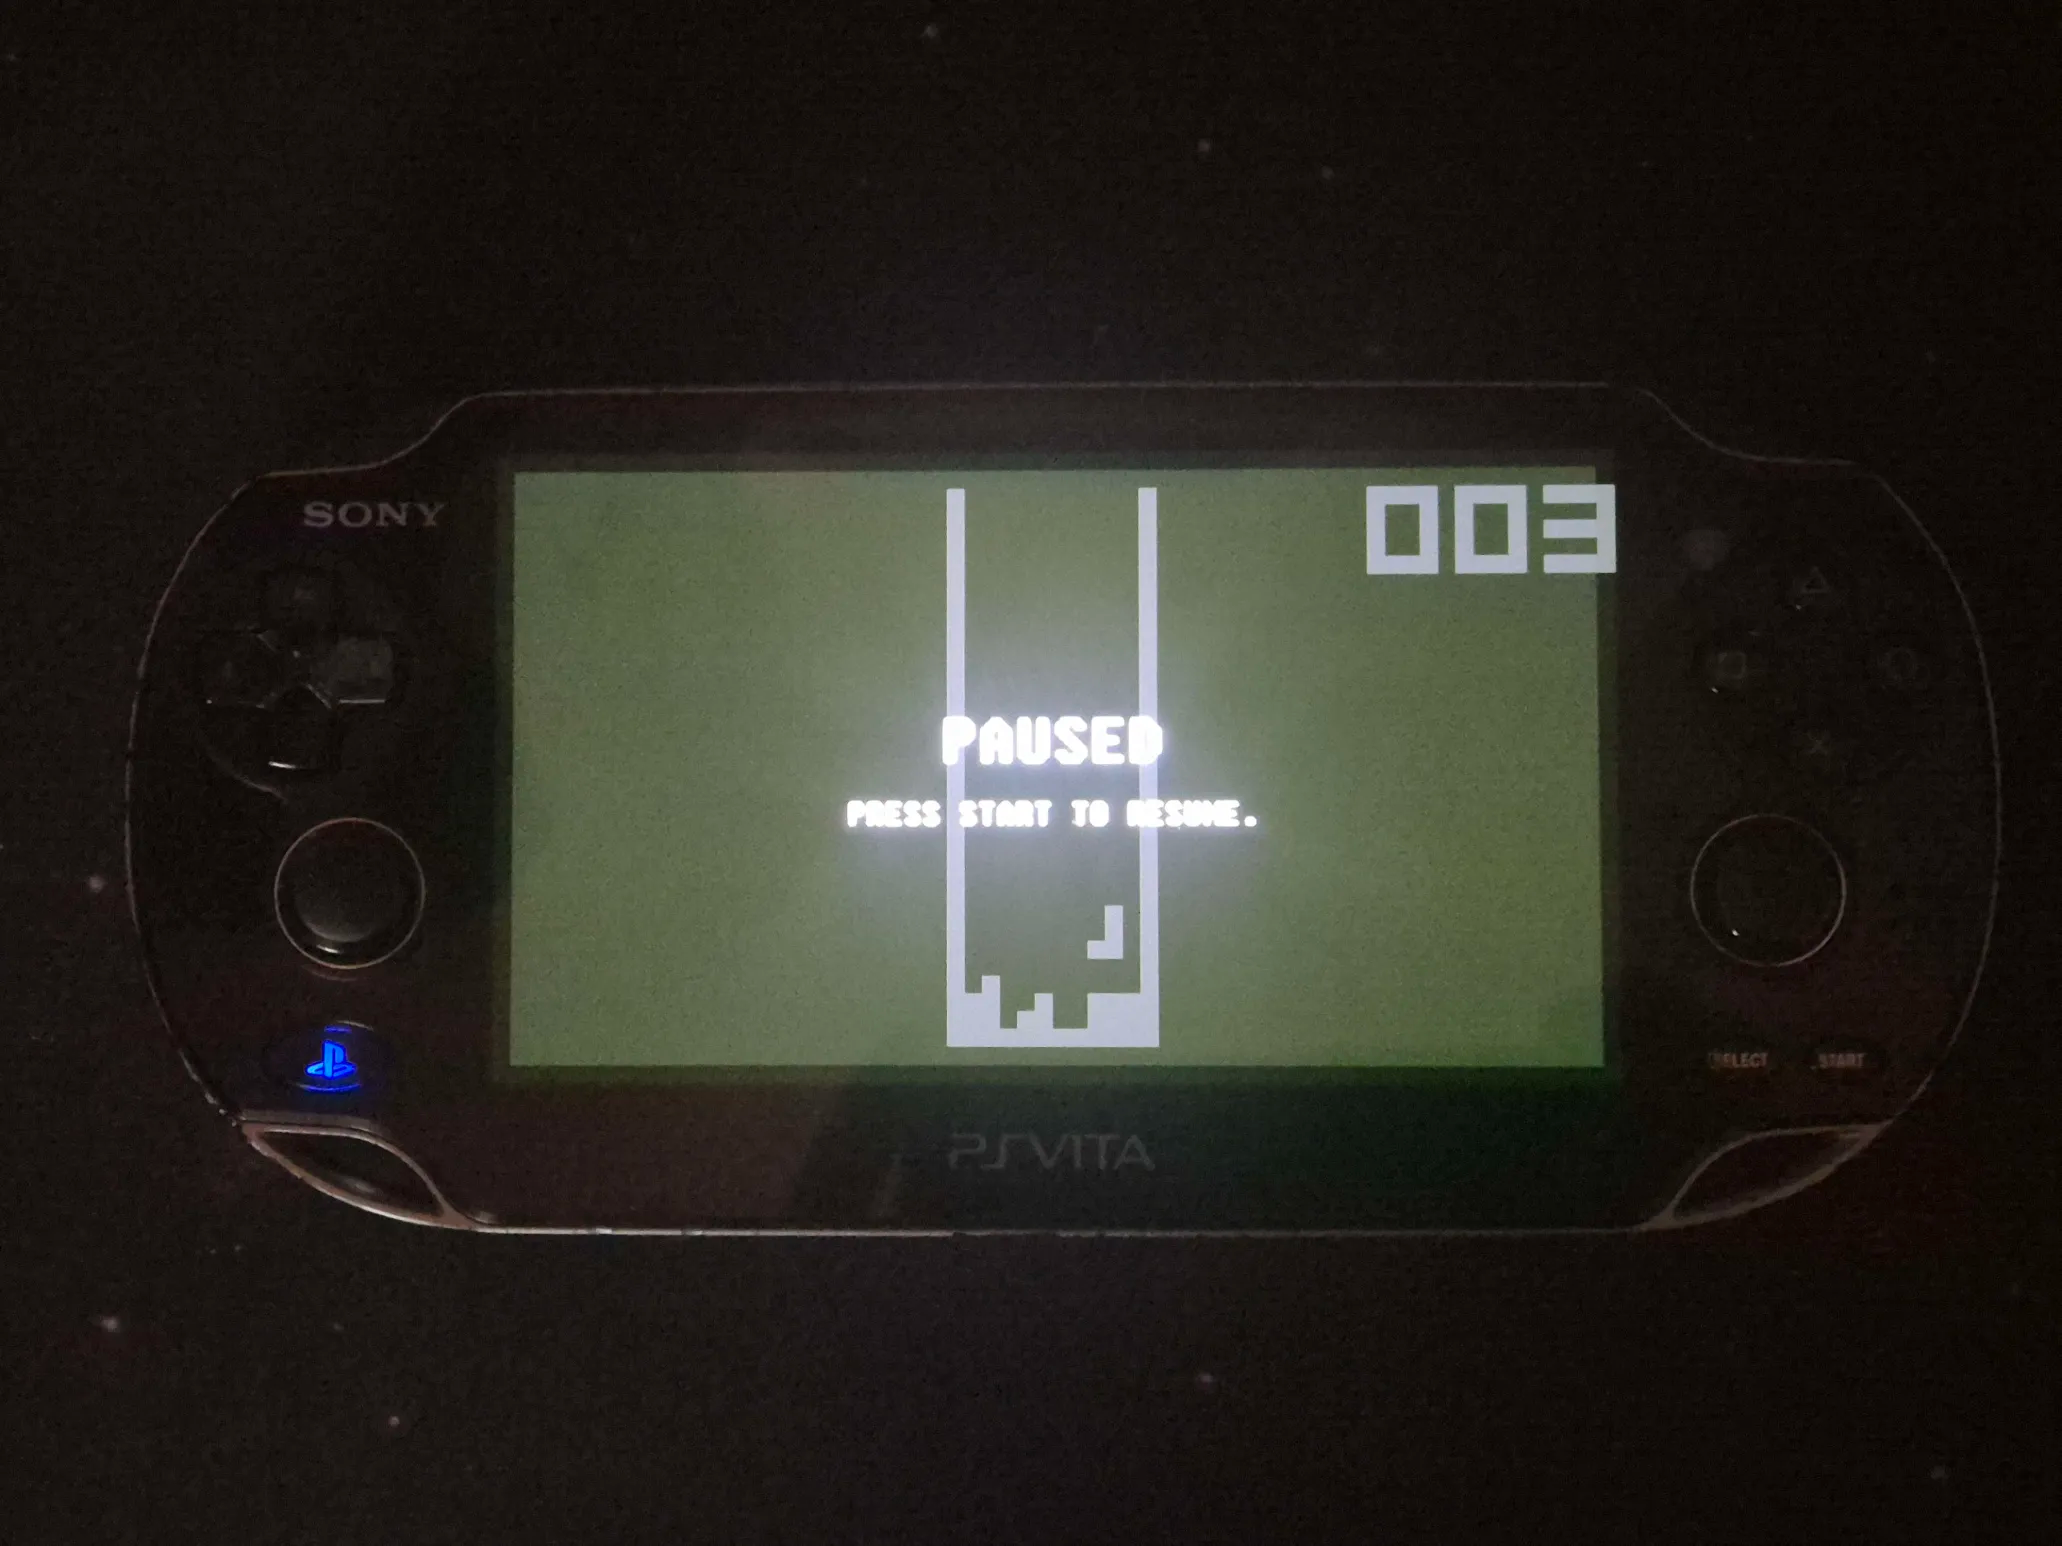
\includegraphics[width=0.75\textwidth]{app/vita}
\captionof{figure}{The app running on a PlayStation Vita system.}
\end{minipage}

\begin{minipage}{\linewidth}
\centering
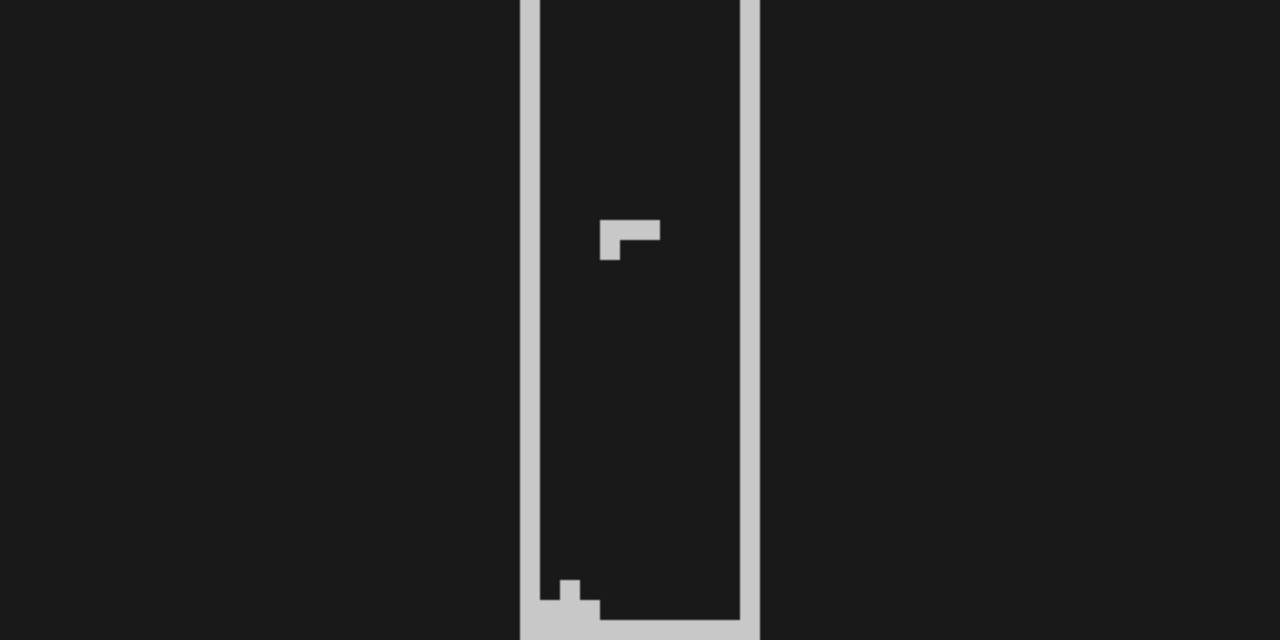
\includegraphics[width=0.66\textwidth]{app/normal}
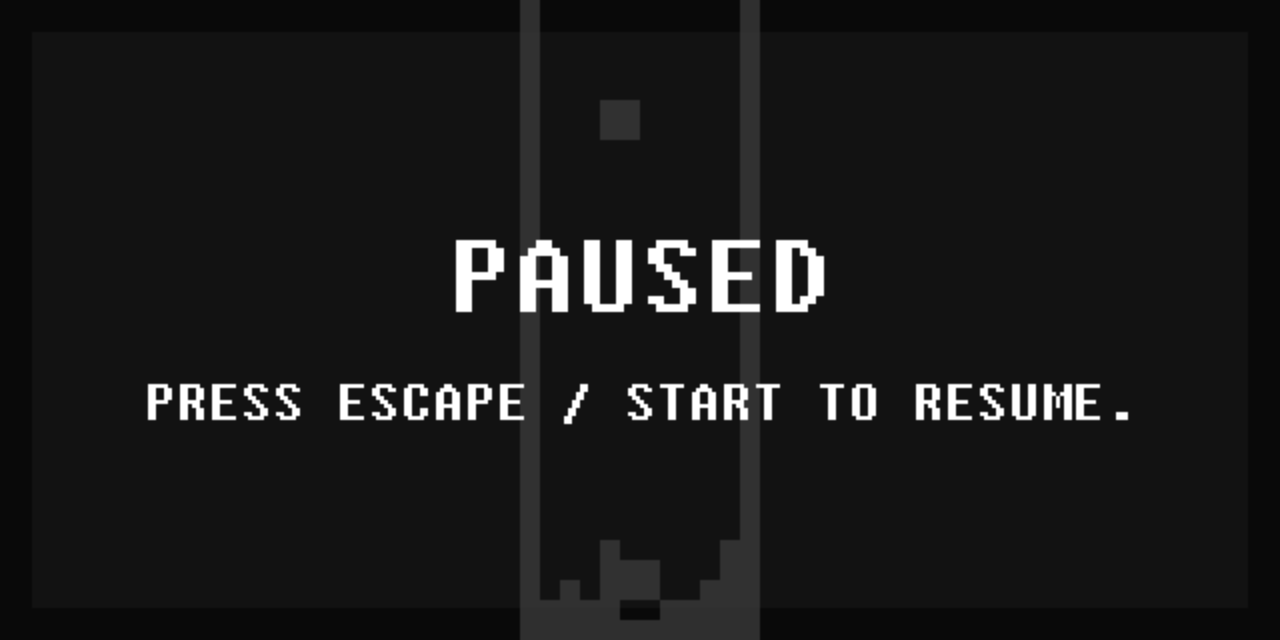
\includegraphics[width=0.66\textwidth]{app/pause}
\captionof{figure}{The app being paused by pressing Escape or Start on a gamepad.}
\end{minipage}